% 
% SBXG Design Document
% 

\documentclass{article}
\usepackage[T1]{fontenc}
\usepackage[utf8]{inputenc}
\usepackage[english]{babel}

\usepackage{hyperref}
\usepackage{mdframed}
\usepackage{tikz}
\usepackage{caption}

\usetikzlibrary{shapes,arrows,positioning}
\tikzstyle{Block} = [draw, rectangle, minimum height=3em, minimum width=3em]
\tikzstyle{Text} = [draw, rectangle]

\newcommand{\email}[1]{%
  \href{mailto:#1}{#1}%
}

\newmdtheoremenv[%
linecolor=black,
frametitlerule=true,
]{requirement}{Requirement}

\title{SBXG Design Document}
\date{}
\author{%
  Jean Guyomarc'h%
  \\Jean-Marc Lacroix%
}

\begin{document}

\maketitle
\tableofcontents
\clearpage

\part{Overall description of SBXG}

SBXG is a build orchestrator that provides means to generate from sources or
foreign binaries a ready-to-flash SD (Secure Digital) card image for embedded
systems.

SBXG orchestrates several components:
\begin{itemize}
\item a toolchain to compile most of the other components;
\item a bootloader builder;
\item a kernel builder;
\item a kernel packager;
\item an initramfs builder for the kernel that may rely on it;
\item a primary rootfs generator;
\item and a filesystem utility to generate the final image which will contain the
  desired components.
\end{itemize}

All of these components can be used individually, or chained together to
generate more complex systems.



\section{Toolchain Retrieving}

The \emph{toolchain} is a suite of software tools that allows to create another
software. When we refer to a toolchain, we refer to a (cross) compiler driver
and its own components (like gcc and the collection programs it relies on).

Since SBXG is primarily targetting embedded platforms, the toolchain will mostly
be arm-flavoured. The different arm architectures will vary in function of the
\emph{processor} embedded on the SoC that ships with an \emph{embedded board}.

We select our toolchains from \url{https://www.linaro.org/}, but custom ones can
of course be provided.

\begin{requirement}
  SBXG is required to fetch an external toolchain or to use an already existing
  one.
\end{requirement}

\begin{center}
  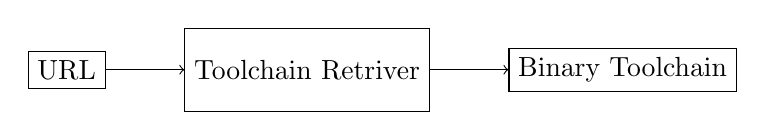
\begin{tikzpicture}
    \node[Block] (component)                      {Toolchain Retriver};
    \node[Text]  (config)    [left=of component]  {URL};
    \node[Text]  (output)    [right=of component] {Binary Toolchain};
    \draw[->] (config)    to (component);
    \draw[->] (component) to (output);
  \end{tikzpicture}
\end{center}


\section{Bootloader Builder Component}

The \emph{bootloader} is the piece of software that is responsible for
bootstrapping the primary kernel which will operate the system. In the embedded
world, which consists mainly of ARM-based SoCs, U-Boot is the most prevalent
bootloader. The bootloader builder provided by SBXG is therefore strongly
oriented towards U-Boot.

\begin{center}
  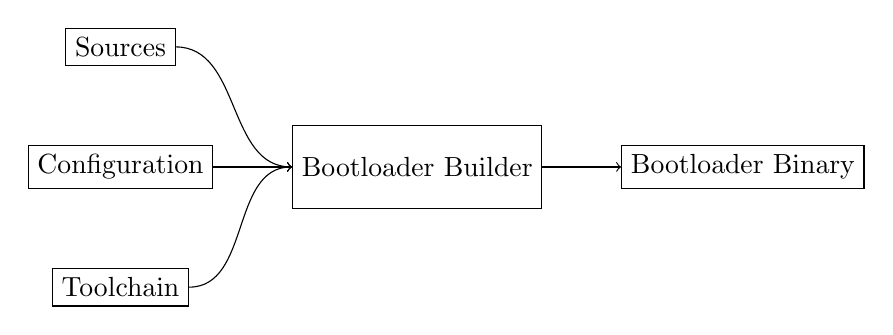
\begin{tikzpicture}
    \node[Block] (component)                      {Bootloader Builder};
    \node[Text]  (config)    [left=of component]  {Configuration};
    \node[Text]  (sources)   [above=of config]    {Sources};
    \node[Text]  (toolchain) [below=of config]    {Toolchain};
    \node[Text]  (output)    [right=of component] {Bootloader Binary};
    \draw[->] (toolchain) to [out=0,in=180] (component);
    \draw[->] (sources)   to [out=0,in=180] (component);
    \draw[->] (config)    to [out=0,in=180] (component);
    \draw[->] (component) to (output);
  \end{tikzpicture}
\end{center}

\begin{requirement}
  SBXG is required to generate an U-Boot image.
\end{requirement}


\section{Kernel Components}

The \emph{kernel} is the software that is responsible for user tasks to execute
on a given hardware. We mostly target the Linux kernel, due to its wide range of
drivers, which make it usable on most of the arm SoCs.

Type I hypervisors, such as Xen or Xvisor are also targeted. When considering
hypervisors more generally (type I or type II), guest kernel images shall also
be generated by SBXG.

\begin{requirement}
  SBXG is required to generate a Kernel image and associated runtime files.
\end{requirement}

We make the distinction between \emph{kernel building} and \emph{kernel
  packaging}. Kernel building consists in generating raw images from the
sources, whereas kernel packaging consists in generating an archive that
contains kernel products which will be integrated within a package manager.

\subsection{Kernel Builder Component}

\begin{center}
  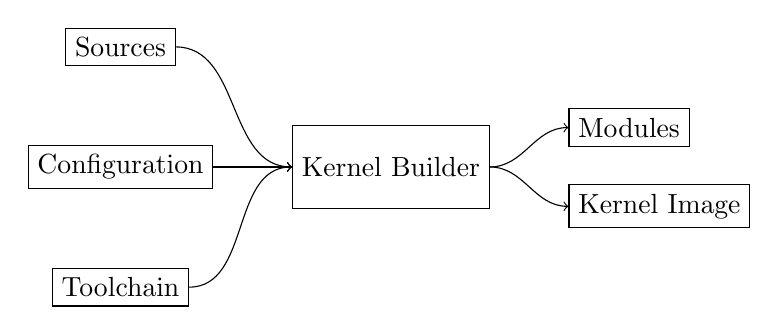
\begin{tikzpicture}
    \node[Block] (component)                      {Kernel Builder};
    \node[Text]  (i_config)    [left=of component]  {Configuration};
    \node[Text]  (i_sources)   [above=of i_config]    {Sources};
    \node[Text]  (i_toolchain) [below=of i_config]    {Toolchain};
    \node[Text]  (o_image)     [right=of component, yshift=-5mm] {Kernel Image};
    \node[Text]  (o_runtime)   [right=of component, yshift=+5mm] {Modules};
    \draw[->] (i_toolchain) to [out=0,in=180] (component);
    \draw[->] (i_sources)   to [out=0,in=180] (component);
    \draw[->] (i_config)    to [out=0,in=180] (component);
    \draw[->] (component)   to [out=0,in=180] (o_image);
    \draw[->] (component)   to [out=0,in=180] (o_runtime);
  \end{tikzpicture}
\end{center}


\subsection{Kernel Packager Component}

\begin{center}
  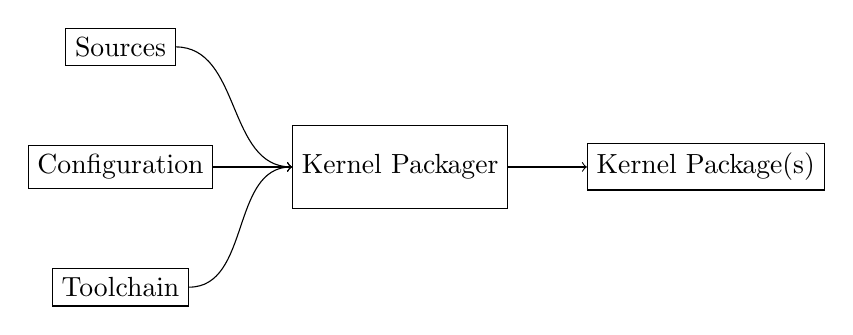
\begin{tikzpicture}
    \node[Block] (component)                        {Kernel Packager};
    \node[Text]  (i_config)    [left=of component]  {Configuration};
    \node[Text]  (i_sources)   [above=of i_config]  {Sources};
    \node[Text]  (i_toolchain) [below=of i_config]  {Toolchain};
    \node[Text]  (o_image)     [right=of component] {Kernel Package(s)};
    \draw[->] (i_toolchain) to [out=0,in=180] (component);
    \draw[->] (i_sources)   to [out=0,in=180] (component);
    \draw[->] (i_config)    to [out=0,in=180] (component);
    \draw[->] (component)   to [out=0,in=180] (o_image);
  \end{tikzpicture}
\end{center}

\subsection{Initramfs Builder Component}

Some kernels may require an \emph{initramfs} to complete their boot process and
to provide a basic shell in case of failure of the system. Systems like
\emph{busybox} allow to generate such software.

\begin{requirement}
  SBXG is required to generate an initramfs on demand. It shall at least support
  the CPIO format.
\end{requirement}

\begin{center}
  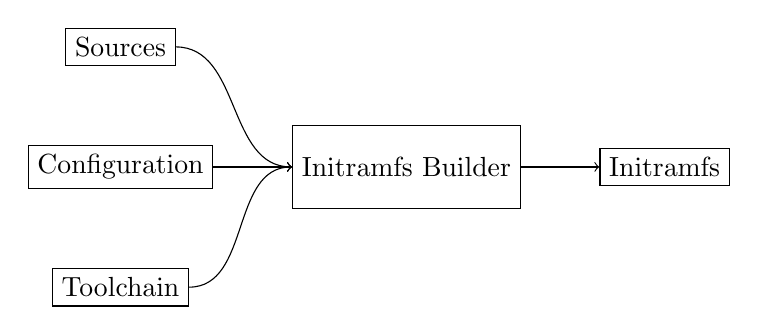
\begin{tikzpicture}
    \node[Block] (component)                        {Initramfs Builder};
    \node[Text]  (i_config)    [left=of component]  {Configuration};
    \node[Text]  (i_sources)   [above=of i_config]  {Sources};
    \node[Text]  (i_toolchain) [below=of i_config]  {Toolchain};
    \node[Text]  (o_image)     [right=of component] {Initramfs};
    \draw[->] (i_toolchain) to [out=0,in=180] (component);
    \draw[->] (i_sources)   to [out=0,in=180] (component);
    \draw[->] (i_config)    to [out=0,in=180] (component);
    \draw[->] (component)   to [out=0,in=180] (o_image);
  \end{tikzpicture}
\end{center}

\section{Rootfs Retriever Component}

The \emph{rootfs} is mounted by the \emph{kernel} and contains the user-land
programs and files that are necessary for the system to operate. Due to the vast
amount of software available, SBXG is not responsible for building a rootfs by
himself. Instead, it shall be able to manipulate an already generated rootfs.

Rootfs can be either build entirely, thanks to software like buildroot or the
Gentoo build system. It can also be retrived as pre-built binaries, thanks to
tools like Deboostrap.

\begin{requirement}
  SBXG is required to integrate an externally generated rootfs in its production
  pipeline.
\end{requirement}

\begin{center}
  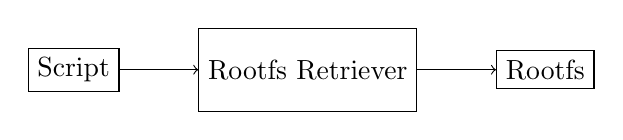
\begin{tikzpicture}
    \node[Block] (component)                      {Rootfs Retriever};
    \node[Text]  (config)    [left=of component]  {Script};
    \node[Text]  (output)    [right=of component] {Rootfs};
    \draw[->] (config)    to (component);
    \draw[->] (component) to (output);
  \end{tikzpicture}
\end{center}

\section{Flash Image Builder Component}

The ultimate goal of SBXG being to provide a ready-to-use flash image, one of
its component shall be responsible in generating a flash image containing the
products of other SBXG components.

\begin{requirement}
  SBXG shall be able to build an image from a collection of products, given an
  associated configuration.
\end{requirement}

\begin{center}
  
\begin{tikzpicture}
    \node[Block] (component)                                  {Image Builder};
    \node[Text]  (config)    [left=of component, yshift=-5mm] {Configuration};
    \node[Text]  (products)  [left=of component, yshift=+5mm] {SBXG Products};
    \node[Text]  (output)    [right=of component]             {SBXG Image};
    \draw[->] (config)    to [out=0,in=180] (component);
    \draw[->] (products)  to [out=0,in=180] (component);
    \draw[->] (component) to (output);
  \end{tikzpicture}
\end{center}


\section{Execution Pipeline}

We define an \emph{execution pipeline} as the sequential execution of one or
several components.

To better illustrate what an execution pipeline, let's consider the following
scenario. A user want to produce a read-to-flash image that contains an U-Boot
image (the bootloader) and a Debian rootfs containing a Linux kernel with its
modules. We just need to chain the components as follows:

\begin{center}
  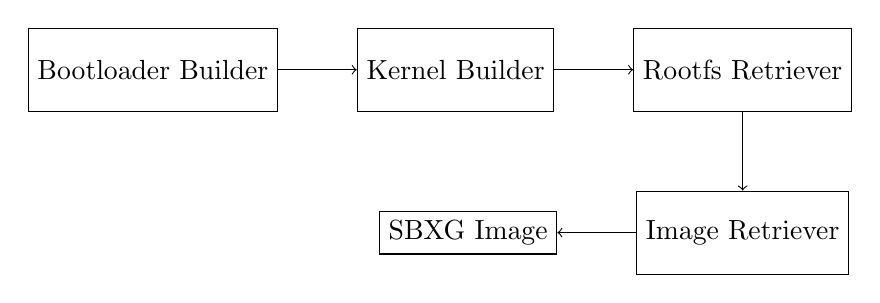
\begin{tikzpicture}
    \node[Block] (uboot)                     {Bootloader Builder};
    \node[Block] (kernel) [right=of uboot]   {Kernel Builder};
    \node[Block] (rootfs) [right=of kernel]  {Rootfs Retriever};
    \node[Block] (image)  [below=of rootfs]  {Image Retriever};
    \node[Text]  (output) [left=of image]    {SBXG Image};
    \draw[->] (uboot)    to (kernel);
    \draw[->] (kernel)  to (rootfs);
    \draw[->] (rootfs) to (image);
    \draw[->] (image) to (output);
  \end{tikzpicture}
  \captionof{figure}{Execution pipeline with four components}
  \label{fig:ex1}
\end{center}

Then, suppose one now want the kernel to use an initramfs. One now can insert
the initramfs builder component in the pipeline:

\begin{center}
  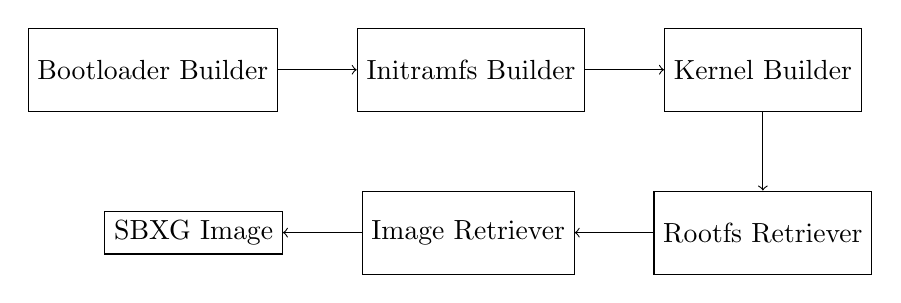
\begin{tikzpicture}
    \node[Block] (uboot)                         {Bootloader Builder};
    \node[Block] (initramfs) [right=of uboot]    {Initramfs Builder};
    \node[Block] (kernel) [right=of initramfs]   {Kernel Builder};
    \node[Block] (rootfs) [below=of kernel]  {Rootfs Retriever};
    \node[Block] (image)  [left=of rootfs]  {Image Retriever};
    \node[Text]  (output) [left=of image]   {SBXG Image};
    \draw[->] (uboot)    to (initramfs);
    \draw[->] (initramfs)    to (kernel);
    \draw[->] (kernel)  to (rootfs);
    \draw[->] (rootfs) to (image);
    \draw[->] (image) to (output);
  \end{tikzpicture}
  \captionof{figure}{Execution pipeline with five components}
\end{center}


This example is simple enough to illustrate how powerful the execution pipeline,
as an architectural element can be. However, the figure was over-simplified, and
it didn't really show the hidden inherent complexity of SBXG. To have an
accurate representation of the pipeline system, one must include the inputs and
outputs of each component in the picture. We will do the exercise based on
\autoref{fig:ex1}.

\end{document}
